\chapterimage{componentes.jpg} % Table of contents heading image
\chapter{Componentes}

Se define componente como el medio a través del cual se realiza una encapsulación a un nivel mayor al de una clase o un paquete, de forma que se introduzcan allí soluciones, y se exporten a través de interfaces, lo cual construye un ecosistema de interacción a través de elementos denominados cajas negras, aquellas con las cuales solo es posible la interacción y no la modificación, todo encaminado a brindar de una mayor seguridad a los módulos Estos componentes son parte de un sistema o un subsistema del mismo. El sistema puede estar formado por uno o varios de éstos. Se tratan de elementos que, a través de algún tipo de asociación o contigüidad, dan lugar a un conjunto uniforme.\nocite{Notas}

Para una aplicación los componentes funcionan como cajas negras, los cuales son elementos que reciben una entrada y según ésta, dan una respuesta de salida sin tener en cuenta cómo es su funcionamiento interno, en otras palabras, de una caja negra será primordial la forma en que interactua con el medio que existe sin hacer relevante los procesos que llevan a cabo.

La implementación de componentes como parte del sistema se hace para evitar que se ha denominado aplicación monolítica, dado que esta describe una única aplicación de software en niveles en los que la interfaz de usuario y código de acceso a datos se combinan en un solo programa de una plataforma única \cite{Pw6AM}.

Las Aplicaciones monolíticas aunque se pueden desarrollar sin problema alguno, tienen bastantes desventajas como por ejemplo:

\begin{itemize}
		\item Requieren mayor hardware en las estaciones de trabajo
		\item Son infinitamente más lentos en el procesamiento de peticiones sencillas
		\item Requiere habilitar el acceso real a la carpeta de datos para todos los usuarios de la aplicación 
		\item Su actualización es más costosa
		\item No permite el acceso en línea desde fuera de la red local o requieren de implementaciones de soluciones de conectividad muy costosa.
		\item Ocupan mayor ancho de banda, provocando congestionamiento en la Red Local.
\end{itemize}

Por esto mismo se tiene como preferencia que las diferentes soluciones se caractericen por la mayor cantidad de componentes como sean requeridos.

\section{Diagrama de componentes}

Un diagrama de componentes es un diagrama de tipo del Lenguaje Unificado de Modelado (UML). Éste representa cómo un sistema de software es dividido en componentes y muestra la interacción entre estos componentes.

Un diagrama de componentes muestra los elementos de un diseño de un sistema de software, permite visualizar la estructura de alto nivel del sistema y el comportamiento del servicio que estos componentes proporcionan y usan a través de interfaces\cite{Pw7DC}.

Para entender estos diagramas, es necesario definir los elementos que posee:
\begin{itemize}
	\item \textbf{Componentes}: Es una parte física del sistema, ya sea un modulo, base de datos, programa externo,etc. 
	\item \textbf{Interfaces}: Es el lazo de unión de varios componentes, puede ser requerida, en cuyo caso representa un grupo de mensajes o llamadas que envía el componente a otros componentes o sistemas externos la cual está diseñada para acoplarse a componentes que proporcionan estas operaciones, o ser proveída, por lo que son aquellas llamadas o mensajes que implementa un componente y puede ser usada por otros componentes o sistemas externos. En general estas interfaces son las que definen el api del componente.
	\item \textbf{Paquetes o sub-sistemas}: Algunas veces varios componentes pueden agruparse en un solo paquete o venir dentro de otros componentes que funcionen como sub-sistemas.
\end{itemize} 

Para nuestra aplicación se han desarrollado tres componentes fundamentales para el correcto funcionamiento de ésta, así entonces, se definen los componentes de Movimientos, persistencia y el componente principal que es el nucleo de la aplicación EconomApp.

\begin{figure}[H]
	\centering
	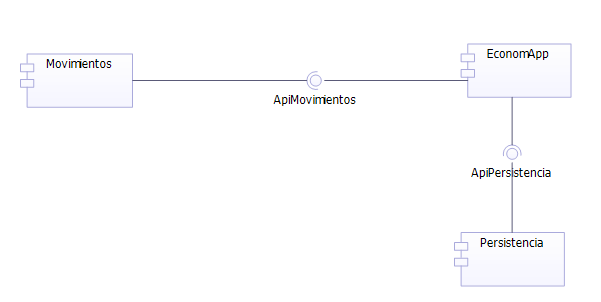
\includegraphics[width=1\linewidth]{parte2/imgs/DiagramaDeComponentes/api}
	\caption{Diagrama de componentes utilizando APIs para su interacción}
	\label{fig:api}
\end{figure}

Para un mayor detalle de cómo funcionan los componentes seleccionados, en la siguiente figura se puede visualizar un diagrama de clases para cada uno de forma particular.

\begin{figure}[H]
	\centering
	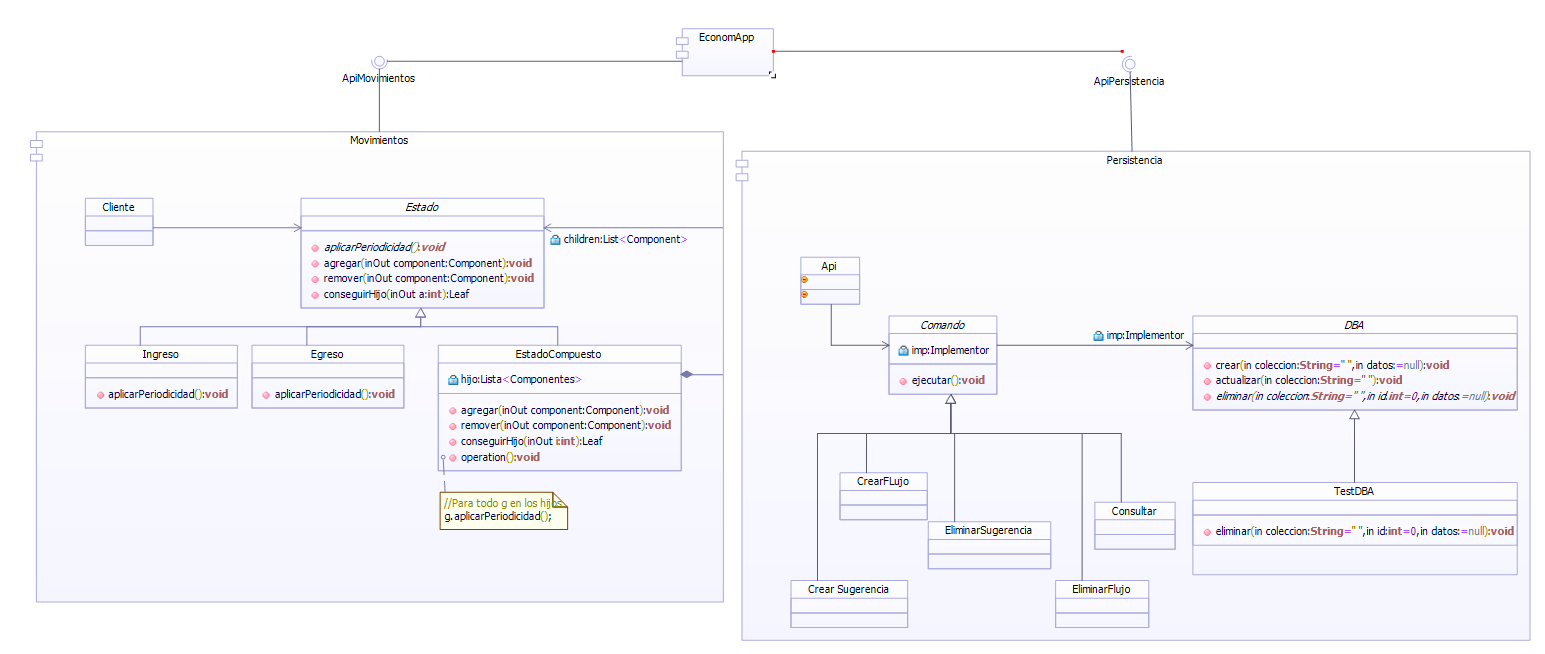
\includegraphics[width=1\linewidth]{parte2/imgs/DiagramaDeComponentes/apiDetallado}
	\caption{Detallado de la estructura interna de los componentes}
	\label{fig:apidetallado}
\end{figure}

Así, el componente de Movimientos se fundamenta en el patrón de Estado, en éste se define la interacción y el cambio de estado de los elementos con los que funcionará el programa, como lo son INGRESO y EGRESO, los cuales heredan de estado. 	

Mientras que en el componente de persistencia se puede apreciar la implementación del patrón Comando, en este componente se manejara todo el tema relacionado con la persistencia del programa, es decir, la base de datos de la que dispone, utilizando el patrón comando para gestionar el CRUD de la base de datos de forma eficiente. 